\documentclass[12pt]{report}
\usepackage{graphicx}
\usepackage{scribe_MG}
\usepackage{amssymb}
\usepackage{graphicx}
\usepackage[mathscr]{eucal}
\usepackage[english]{babel}
\usepackage[utf8]{inputenc}  %encodage du fichier
\usepackage[T1]{fontenc}


\usepackage{placeins} 

\newcommand\independent{\protect\mathpalette{\protect\independenT}{\perp}}
\def\independenT#1#2{\mathrel{\rlap{$#1#2$}\mkern2mu{#1#2}}} 

\newtheorem{remarque}{Remark}[section]
\newtheorem{exemple}{Example}[section]

\begin{document}
\coursetitle{K-means, EM, Gaussian Mixture, Graph Theory}
\semester{2013/2014}
\lecturer{Francis Bach} \scribe{Marie d'Autume, Jean-Baptiste Alayrac}
\lecturenumber{3} \lecturedate{October 16th}

\maketitle

\begin{danger}
 
 To talk about estimation of "hidden" parameters, French speaking people and English speaking people use different terms which can lead to some confusions. Within a supervised framework, English people would prefer to use the term \textit{classification} whereas the French use the term \textit{discrimination}. Within an unsupervised context, English people would rather use the term \textit{clustering}, whereas French people would use \textit{classification} or \textit{classification non-supervis\'ee}. In the following we will only use the English terms.

\end{danger}

\section{$K$-means}

$K$- means clustering is a method of vector quantization. $K$-means clustering is an algorithm
of alternate minimization that aims at partitioning $n$ observations into $K$ clusters in which each observation belongs to the cluster with the nearest mean, serving as a prototype to the cluster (see Figure \ref{kmeans01}).


\begin{figure}[ht]
  \label{kmeans01}
  \centering
  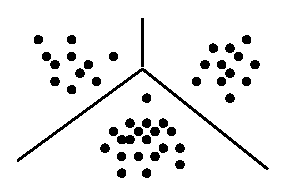
\includegraphics[width=5cm]{./figures/kmeans01.eps}
  \caption{Clustering on a 2D point data set with 3 clusters.}
\end{figure}

\subsection{Notations and notion of Distortion}

We will use the following notations: 
\begin{itemize}
\item $x_i \in  \mathbb{R}^p $, $i\in\{1,...,n\}$ are the observations we want to partition.
\item $\mu_k \in \mathbb{R}^p$, $k\in\{1,...,K\}$ are the means where $\mu_k$ is the center of the cluster $k$. We will denote $\mu$ the associated matrix.
\item $z_i^k$ are indicator variables associated to  $x_i$ such that $z_i^k=1$ if $x_i$ belongs to the cluster $k$, $z_i^k=0$ otherwise. $z$ is the matrix which components are equal to $z_i^k$.
\end{itemize}

Finally, we define the \textit{distortion} $J(\mu,z)$ by:
$$J(\mu,z)=\sum_{i=1}^n \sum_{k=1}^K z_i^k \| x_i-\mu_k \|^2.$$

\subsection{Algorithm}

The aim of the algorithm is to minimize $J(\mu,z)$. To do so we proceed with an alternating minimization :

\begin{itemize}
\item Step 0 : We choose a vector $\mu$
\item Step 1 : we minimize $J$ with respect to $z$ :  $z_i^k=1$ if $\parallel x_i-\mu_k\parallel^2 = \min_s\parallel x_i-\mu_s\parallel^2$, in other words we associate to $x_i$ the nearest center $\mu_k$.
\item Step 2 : we minimize $J$ with respect to $\mu$ :
  $\mu_k=\frac{\sum_i z_i^k x_i}{\sum_i z_i^k}$.
\item Step 3 : we come back to step 1 until convergence.
\end{itemize}

\begin{remarque} 
The step of minimization with respect to $z$ is equivalent to allocating the $x_i$ in the Voronoi cells which centers are the $\mu_k$.
\end{remarque}

\begin{remarque} 
During the step of minimization with respect to $\mu$, $\mu_k$ is obtained by setting to zero the $k$-th coordinate of the gradient of $J$ with respect to $\mu$. Indeed we can easily see that :
\begin{equation*}
\nabla_{\mu_k }J = -2\sum_i z_i^k(x_i-\mu_k)
\end{equation*}

\end{remarque}

\subsection{Convergence and Initialization}

We can show that this algorithm converges in a finite number of iterations. Therefore the convergence could be local, thus it introduces the problem of initialization. 

A classic method is use of random restarts. It consists in choosing several random vectors $\mu$, computing the algorithm for each case and finally keeping the partition which minimizes the distortion. Thus we hope that at least one of the local minimum is close enough to a global minimum.

One other well known method is the $K$-means$++$ algorithm, which aims at correcting a major theoretic shortcomings of the $K$-means algorithm : the approximation found can be arbitrarily bad with respect to the objective function compared to the optimal clustering.
 
The $K$-means$++$ algorithm addresses this obstacles by specifying a procedure to initialize the cluster centers before proceeding with the standard $K$-means optimization iterations. With the $K$-means $++$ initialization, the algorithm is guaranteed to find a solution that is $O(\log K)$ competitive to the optimal $K$-means solution. 
\newpage
The intuition behind this approach is that it is a clever thing to well spread out the $K$ initial cluster centers. At each iteration of the algorithm we will build a new center. We will repeat the algorithm until we  have $K$ centers. Here are the steps of the algorithm : 

\begin{itemize}
\item Step 0 : First initiate the algorithm by choosing the first center uniformly at random among the data points. 

\item Step 1: For each data point $x_i$ of your data set, compute the distance between $x_i$ and the nearest center that has already been chosen. We denote this distance $D_{\mu_t}(x_i)$ where $\mu_t$ is specified to recall that we are minimizing over the current chosen centers.
 
\item Step 2: Choose one new data point at random as a new center, but now using a weighted probability distribution where a point $x_i$ is chosen with probability proportional to $D_{\mu_t}(x_i)^2$.

\item Step 3 : Repeat Step 1 and Step 2 until $K$ centers have been chosen.

\end{itemize}

We see that we have now built $K$ vectors with respect to our first intuition which was to well spread out the centers (because we used a well chosen weighted probability). We can now use those vectors as the initialization of our standard $K$-means algorithm.  

More details can be found on the $K$-means$++$ algorithm in [A].

\vspace*{1cm}

[A] Arthur, D. and Vassilvitskii, S. (2007). k-means++: the advantages of careful seeding. Proceedings of the eighteenth annual ACM-SIAM symposium on Discrete algorithms.


\subsection{Choice of $K$}

It is important to point out that the choice of $K$ is not universal. Indeed, we see that if we increase $K$, the distortion $J$ decreases, until it reaches $0$ when $K=n$, that is to say when each data point is the center of its own center. To address this issue one solution could be to add to $J$ a penalty over $K$. Usually it takes the following form : 
$$ J(\mu,z,K)=\sum_{i=1}^n \sum_{k=1}^K z_i^k \| x_i-\mu_k \|^2 + \lambda K$$

But again the choice of the penalty is arbitrary.
\newpage
\subsection{Other problems}
We can also point out that $K$-means will work pretty well when the width of the different clusters are similar, for example if we deal with spheres. But clustering by $K$-means could also be disappointing in some cases such as the example given in Figure \ref{kmeansissue}.

\begin{figure}[ht]
  
  \centering
  \includegraphics[width=10cm]{./figures/kmeansissue.eps}
  \caption{\label{kmeansissue} Example where $K$- means does not provide a satisfactory clustering result}
\end{figure}

Using Gaussian mixtures provides a way to avoid this problem (see next section).

\section{EM : Expectation Maximization}

The Expectation-maximization  (EM) algorithm is an iterative method for finding maximum likelihood estimates of parameters in statistical models, where the models depend on unobserved latent or hidden variables $z$. Latent variables are variables that are not directly observed but are rather inferred from other variables that are observed.

Previous algorithms aimed at estimating the parameter $\theta$ that maximized the likelihood of $p_{\theta}(x)$, where $x$ is the vector of observed variables.

Here it is a little bit different. Indeed we have now :
\\ \\
\textit{Assumption} : $(x,z)$ are random variables where $x$ is observed (our data) and $z$ is non observed (unknown cluster center for example).
\begin{center}
$ p_{\theta}(x,z)$ : joint density depending on a parameter $\theta$ (the model)
\end{center}
\textit{The goal} : to maximize the following probability  :
\begin{equation*}
\max_{\theta} p_{\theta}(x) = \sum_zp_{\theta}(x,z).
\end{equation*}
We can already infer that, because of the sum, the problem should be slightly more difficult than before. Indeed, taking the $\log$ of our probability would not lead to a simple convex problem. In the following we will see that EM is a method to solve those kind s of problems.

\subsection{Example}

Let's present a simple example to illustrate what we just said. The probability density represented on Figure \ref{EM01} is akin to an average of two Gaussians. Thus, it is natural to use a mixture model and to introduce an hidden variable $z$, following a Bernoulli distribution defining which Gaussian the point is sampled from.

\begin{figure}[ht]
  \label{EM01}
  \centering
  \includegraphics[width=8cm]{./figures/EM01.eps}
  \caption{Average of two probability distributions of two Gaussian for which it is natural to introduce a mixture model}
\end{figure}

Thus we have : $z\in\{1,2\}$ and $x|z = i \sim
\mathcal{N}(\mu_i,\Sigma_i)$. The density $p(x)$ is a convex combination of normal density:
$$p(x)=p(x,z=1)+p(x,z=2)=p(x|z=1)p(z=1)+p(x|z=2)p(z=2)$$

It is a mixture model. It represents a simple way to model complicated phenomena. 

\subsection{Objective: maximum likelihood}

Let $z$  be the hidden variables and $x$ be the observed data. We make the assumption that the $x_i$, $i\in\{1,...,n\}$ are i.i.d..

As we mentioned it in the introduction the aim is to maximize the likelihood
$$p_{\theta}(x)= \sum_{z}p_{\theta}(x,z)$$
$$\log p_{\theta}(x)= \log \sum_{z}p_{\theta}(x,z)$$.

Note that in practice, we often have $(x,z) = (x_1,z_1,\dots,x_n,z_n)$ where each pair $(x_i,y_i)$ is i.i.d. In this situation we have
$\log p_{\theta}(x)= \sum_{i=1}^n \log \sum_{z_i} p_{\theta}(x_i,z_i)$.

There is at least two ways to solve this problem:
\begin{enumerate}
\item By a direct way, if we can, by a gradient ascent for example.
\item By using the EM algorithm.
\end{enumerate}

\subsection{Jensen's Inequality}
We will use the following properties :
\begin{enumerate}
\item if $f:\mathbb{R} \rightarrow \mathbb{R}$ is convex and if $X$ is an integrable random variable  :
  $$\mathbb{E}_X(f(X))\geq f(\mathbb{E}_X(X))$$
\item if $f:\mathbb{R} \rightarrow \mathbb{R}$ is strictly convex, we have equality in the previous inequality if and only if 
 $X$ = constant a.s.
\end{enumerate}

\subsection{EM algorithm}

We introduce the function $q(z)$
such that $q(z) \geq 0$ and $\sum_zq(z)=1$ in the expression of the likelihood. Thus we have :
\begin{eqnarray*}
  \log p_{\theta}(x) &=& \log \sum_z p_{\theta}(x,z)\\
  &=& \log \sum_z \left(\frac{p_{\theta}(x,z)}{q(z)} \right) q(z) \\
  &\geq& \sum_z q(z) \log \frac{p_{\theta}(x,z)}{q(z)},\textrm{ by the Jensen's inequality because $\log$ is concave}\\
  &=& \sum_z q(z) \log p_{\theta}(x,z) - \sum_z q(z) \log q(z)\\
  &=& \mathcal{L}(q,\theta)
\end{eqnarray*}

with equality iff $q(z)=\frac{p_{\theta}(x,z)}{\sum_{z'}
  p_{\theta}(x,z')}=p_{\theta}(z|x)$ (by strict concavity of the logarithm).

\begin{proposition} $\forall \theta$, $\forall q$ $\log p_{\theta}(x)
\geq \mathcal{L}(q,\theta)$ with equality if and only if
$q(z)=p_{\theta}(z|x)$.
\end{proposition}

\begin{remarque} We have introduced an auxiliary function $\mathcal{L}(q,\theta)$ that is always below the function 
$\log(p_{\theta}(x))$
\end{remarque}

%figure

\paragraph{EM algorithm}

is an algorithm of alternate maximization with respect to $q$ and $\theta$.

We initialize $\theta_0$, then we iterate for $t>0$, by alternating the following steps until convergence:
\begin{itemize}
\item  $q_{t+1} \in \operatorname{arg\,max}_q(\mathcal{L}(q,\theta_t))$
\item  $\theta_{t+1} \in \operatorname{arg\,max}_{\theta}(\mathcal{L}(q_{t+1},\theta))$
\end{itemize}

\paragraph{Algorithm properties}

\begin{itemize}
\item It is an ascent algorithm, indeed it goes up in term of likelihood (compare to before where we were descending along the distortion) : $$\forall t
  \log(p_{\theta_t})\geq \log(p_{\theta_{t-1}})$$
\item The sequence of log-likelihoods converges.
\item It does not converge to a global maximum but rather to a local maximum because we are dealing here with a non-convex problem.   An illustration is given in Figure \ref{EMIllustration}.
\begin{figure}[ht]  
  \centering
  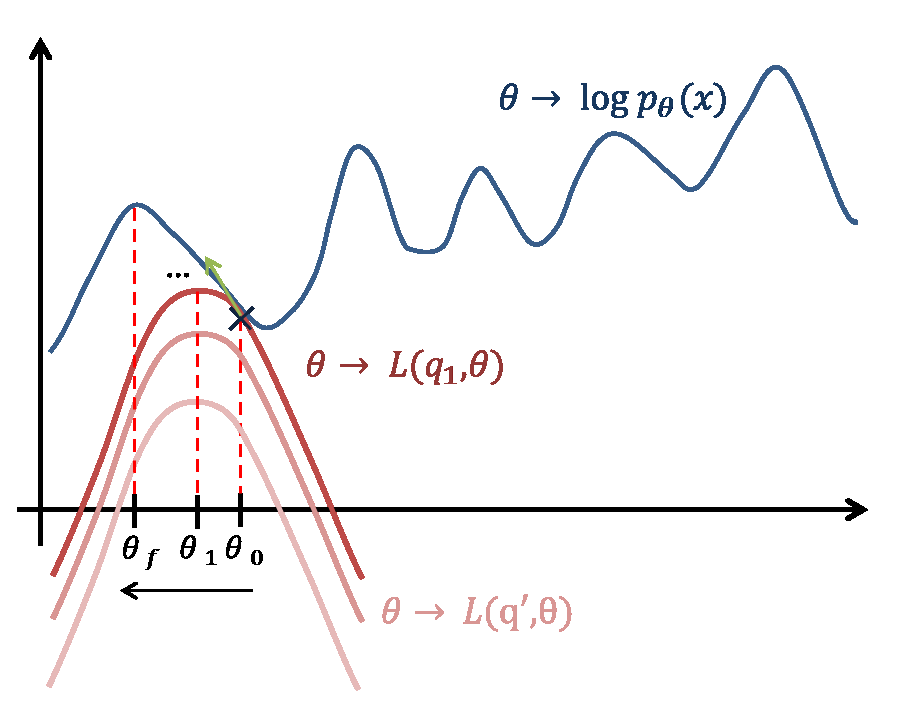
\includegraphics[width=10cm]{./figures/illustrationem.eps}
  \caption{\label{EMIllustration}An illustration of the EM algorithm that converges to a local minimum.}
\end{figure}
\item As it was already the case for $K$-means, we reiterate the result in order to be more confident. Then we keep the one with the highest likelihood.  
\end{itemize}

\paragraph{Initialization}

Because EM gives a local maximum, it is clever to choose a $\theta_0$ relatively close to the final solution. For Gaussian mixtures, it is quite usual to initiate EM by a $K$-means. The solution of $K$-means gives the $\theta_0$ and a large variance is used.

\newpage
\paragraph{The EM recipe}

Let's recall the initial goal of the algorithm. The goal is to maximize the \textit{incomplete} likelihood $\log(p_{\theta}(x))$. To do so we want to maximize the following function which is always inferior to $\log(p_{\theta}(x))$ :
$$ \mathcal{L}(q,\theta) = \sum_z q(z) \log p_{\theta}(x,z) - \sum_z q(z) \log q(z).$$
\begin{enumerate}
\item Compute the probability of Z given X : $p_{\theta_t}(z|x)$ (Corresponding to $q_{t+1} =\operatorname{arg\,max}_q\mathcal{L}(q,\theta_t)$)
\item Write the \textit{complete} likelihood $l_c =
  \log(p_{\theta_t}(x,z))$.
\item \textbf{E-Step} : calculate the expected value of the complete log likelihood function, with respect to the conditional distribution of $Z$ given $X$ under the current estimate of the parameter $\theta_t$ :
  $\mathbb{E}_{Z|X}(l_c)$.
\item \textbf{M-Step} : find $\theta_{t+1}$ by maximizing $ \mathcal{L}(q_{t+1},\theta)$ with respect to $\theta$.
\end{enumerate}


\subsection{Gaussian Mixture}

Let $(x_i,z_i)$ be a couple, for $i \in \{1,...,n\}$ with $x_i \in \mathbb{R}^p$, $z_i \sim \mathcal{M}(1,\pi_1,...,\pi_k)$  and
$(x_i|z_i=j) \sim \mathcal{N}(\mu_j, \Sigma_j)$. Here we have $\theta = (\pi, \mu, \Sigma)$.

\paragraph{Calculation of $p_{\theta}(z|x)$}

We write $p_{\theta}(x_i)$ :

\begin{eqnarray*}
  p_\theta(x_i) & = & \sum_{z_i} p_\theta(x_i,z_i) = \sum_{z_i} p_\theta(x_i|z_i)p_\theta(z_i)\\
  & = & \sum_{j=1}^k p_\theta(x_i|z_i=j)p_\theta(z_i=j)\\
\end{eqnarray*}

Then we use the Bayes formula to estimate $p_{\theta}(z|x)$ :

\begin{eqnarray*}
p_\theta(z_i=j|x_i) & = & \frac{p_\theta(x_i|z_i=j)p_\theta(z_i=j)}{p_\theta(x_i)}\\
&( \varpropto & p_\theta(x_i|z_i=q)p_\theta(z_i=q) )\\
& = & \frac{\pi_j\mathcal{N}(x_i|\mu_j,\Sigma_j)}{\sum_{j'}\pi_{j'}\mathcal{N}(x_i|\mu_j',\Sigma_j')}\\
& = & \tau_i^j(\theta).
\end{eqnarray*}

We recall that
$\mathcal{N}(x_i|\mu,\Sigma)=\frac{1}{(2\pi)^{\frac{d}{2}}|\Sigma|^{\frac{1}{2}}}\exp(-\frac{1}{2}(x-\mu)^T
\Sigma^{-1}(x-\mu))$.

\newpage
Suppose that we are at the $t$-th iteration of the algorithm.
\paragraph{Complete likelihood} Let's write the complete likelihood of the problem.

\begin{eqnarray*}
l_{c,t} = \log p_{\theta_t}(x,z) & = & \sum_{i=1}^n \log
p_{\theta_t}(x_i,z_i)\\
& = & \sum_{i=1}^n \log (p_{\theta_t}(z_i)p_{\theta_t}(x_i|z_i))\\
& = & \sum_{i=1}^n \log(p_{\theta_t}(z_i)) + \log(p_{\theta_t}(x_i|z_i))\\
& = & \sum_{i=1}^n \sum_{j=1}^k z^j_i \log(\pi_{j,t}) + \sum_{i=1}^n \sum_{j=1}^k z_i^j\log(\mathcal{N}(x_i|\mu_{j,t},\Sigma_{j,t}))
\end{eqnarray*}
where $z^j_i \in \{0,1\}$ with $z^j_i = 1$ if $z_i = j$ and $0$ otherwise. 
\paragraph{E-Step} We can now write the expectation of the previous quantity with respect to the conditional distribution of $Z$ given $X$. In fact it is equivalent to replace $z^j_i$ by $\mathbb{E}_{Z|X}(z^j_i)=p_{\theta_t}(z=j|x_i) = \tau^j_i(\theta_t)$. 
Indeed, the other terms of the sum are constant from the point of view of the conditional probability of $Z$ given $X$, and we finally obtain $\mathbb{E}_{Z|X}(l_{c,t})$. Since the value of $\theta_t$ will be fixed during the M-step, we drop the dependence on $\theta_t$ and write $\tau^j_i$. 

\paragraph{M-Step}
For the M-step, we this need to maximize:

\begin{equation*}
\sum_{i=1}^n \sum_{j=1}^k \tau_i^j \log(\pi_{j,t}) + \sum_{i=1}^n \sum_{j=1}^k \tau_i^j \left[\log(\frac{1}{(2\pi)^{\frac{k}{2}}})+\log(\frac{1}{|\Sigma_{j,t}|^{\frac{1}{2}}}) 
  - \frac{1}{2}(x_i-\mu_{j,t})^T \Sigma_{j,t}^{-1} (x_i-\mu_{j,t})) \right]  
\end{equation*}


We want to maximize the previous equation with respect to $\theta_t=(\Pi_t,\mu_t,\Sigma_t)$

As the sum is separated into two terms independent along the variables we can first maximize with respect to $\pi_t$ :

$$\max_{\Pi}\sum_{j=1}^{k}\sum_{i=1}^{n}
\tau_{i}^{j} \log\pi_{j}\ \ \ \Rightarrow\ \ \ \pi_{j,t+1}=\dfrac{\sum_{i=1}^{n}
\tau_{i}^{j} }{\sum_{i=1}^{n}\sum_{j'=1}^{k}
\tau_{i}^{j'} }=\dfrac{1}{n}\sum_{i=1}^{n}
\tau_{i}^{j} $$

We can now maximize with respect to $\mu_t$ and $\Sigma_t$. By computing the gradient along the $\mu_{j,t}$ and along the $\Sigma_{j,t}$, we obtain :

$$ \mu_{j,t+1}=\frac{\sum_i \tau_i^j x_i}{\sum_i \tau_i^j}$$

$$\Sigma_{j,t+1}=\frac{\sum_i
  \tau_i^j (x_i-\mu_{j,t+1})(x_i-\mu_{j,t+1})^T}{\sum_i \tau_i^j }$$

The M-step in the EM algorithm  corresponds  to the estimation of means step in K-means. Note that the value of $\tau_i^j$ in the expressions above are taken for the parameter values of the previous iterate, i.e., $ \tau_i^j =  \tau_i^j(\theta_t)$.

\paragraph{Possible forms for $\Sigma_{j}$}
\begin{itemize}
\item isotropic: $\Sigma_{j}=\sigma^{2}_{j}
\mathrm{Id}$, 1 parameter, the cluster is a sphere.
\item diagonal: $\Sigma_{j}$ is a diagonal matrix, $d$ parameters, the cluster is an ellipse oriented along  the axis.
\item general: $\Sigma_{j}$, $\frac{d(d+1)}{2}$ parameters, the cluster is an ellipse.
\end{itemize}

\section{Graph theory}

\subsection{Graph}

\begin{definition}[graph] 
A \emph{graph} is a pair $G = (V, E)$ comprising a set $V$ of vertices or nodes together with a set $E\subset V\times V$ of edges or arcs, which are 2-element subsets of $V$. 

\end{definition}

\begin{remarque} In this course we only consider graphs without self-loop.
\end{remarque}

\subsection{Undirected graphs}

\begin{definition}[undirected graph]
  $G=(V,E)$ is an \emph{} if $\forall (u,v)\in
  V\times V$ with $u \neq v$ we have: $$(u,v)\in E \Longleftrightarrow (v,u)
  \in E$$ (Figure \ref{graph01}).
\end{definition}

\begin{figure}[ht]
  \centering
  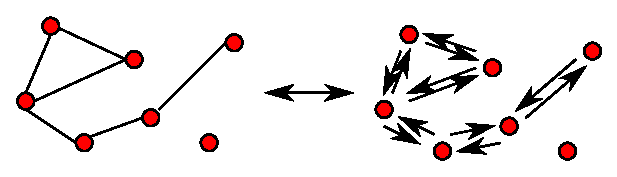
\includegraphics[width=5cm]{./figures/graph01.eps}
  \caption{two different ways to represent an undirected graph}
 \label{graph01}
 \end{figure}
\FloatBarrier

\begin{definition}[neighbour] We 
  define $\mathcal{N}(u)$, the set of the \emph{neighbours} of $u$, as  $$\mathcal{N}(u)=\{ v\in V, (v,u)\in E \}$$ (Figure \ref{graph02}).
\end{definition}

\begin{figure}[ht]
  \centering
  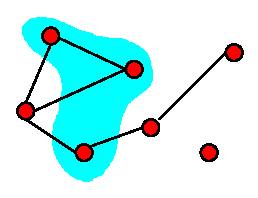
\includegraphics[width=5cm]{./figures/graph02.eps}
  \caption{A vertex and its neighbours}
  \label{graph02}
\end{figure}

\FloatBarrier

\begin{definition}[clique]
  A totally connected subset of vertices  or a singleton is called a \emph{clique} (Figure \ref{graph03}).
\end{definition}

\begin{figure}[ht]
    \centering
  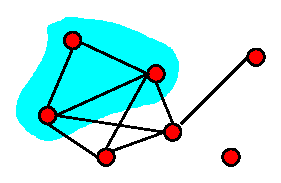
\includegraphics[width=5cm]{./figures/graph03.eps}
  \caption{A clique.}
\label{graph03}
\end{figure}
\FloatBarrier

\begin{definition}[maximal clique]
 A \emph{maximal clique}, $C$, is a clique which is  maximal for the inclusion order: $$\nexists v
  \in V: v \notin C  \ \mathrm{and}\ v \cup C \ \mathrm{is \ a\  clique.} $$ (Figure
  \ref{graph04}).
\end{definition}

\begin{figure}[!ht]
  \centering
  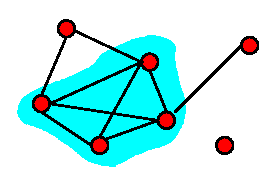
\includegraphics[width=5cm]{./figures/graph04.eps}
  \caption{A maximal clique}
  \label{graph04}
\end{figure}

\FloatBarrier
\begin{definition}[path]
 A  \emph{path} is  a sequence of connected vertices that are globally distinct (Figure \ref{graph05}).
\end{definition}

\begin{figure}[ht]
  \centering
  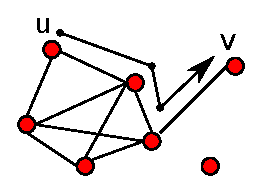
\includegraphics[width=5cm]{./figures/graph05.eps}
  \caption{A path from $u$ to $v$.}
 \label{graph05}
 \end{figure}
\FloatBarrier

\begin{definition}[cycle]
 A \emph{cycle} is a sequence of vertices $(v_{0},\ldots,v_{k})$ such that: 
 \begin{itemize}
 \item $v_{0}=v_{k}$
 \item $\forall j,(v_{j},v_{j+1})\in E$
 \item $\forall i,j, v_{i}\neq v_{j}\ \mathrm{if}\ \lbrace i,j\rbrace\neq\lbrace 1,k\rbrace$
 \end{itemize}
\end{definition}

\begin{definition}
  Let $A$, $B$, $C$ be distinct subsets of $V$. $C$ \emph{separates} $A$ and
  $B$ if all paths from $A$ to $B$ go through $C$ (Figure
  \ref{graph06}).
\end{definition}

\FloatBarrier
\begin{figure}[ht]
  \centering
  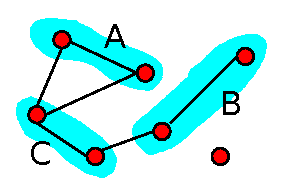
\includegraphics[width=5cm]{./figures/graph06.eps}
  \caption{$C$ separates $A$ and $B$.}
  \label{graph06}
\end{figure}

\begin{definition}[connected component]
  A \emph{connected component} is a subgraph induced by the equivalence class of the relation $uRv\Leftrightarrow\exists$ path from $u$ to $v$ (Figure \ref{graph07}).
\end{definition}

\begin{figure}[ht]
  \centering
  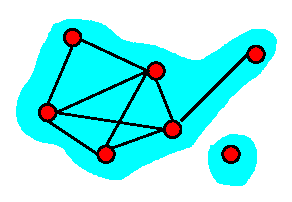
\includegraphics[width=5cm]{./figures/graph07.eps}
  \caption{A graph with 2 connected components}
 \label{graph07}
 \end{figure}

\FloatBarrier
In this course we will consider there is only one connected component. Otherwise we deal with them independently.


\subsection{Oriented graphs}

\begin{definition}[parent]
 $v$ is a \emph{parent} of $u$ if $(v,u)\in E$
\end{definition}

\begin{definition}[children]
  $v$ is a \emph{children} of $u$ if $(u,v)\in E$
\end{definition}

\begin{definition}[ancestor]
  $v$ is an \emph{ancestor} of $u$ if there exists a path from $u$ to $v$.
\end{definition}

\begin{definition}[descendant]
  $v$ is a \emph{descendant} of $u$ if there exists a path from $u$ to $v$
\end{definition}

\begin{definition}[cycle]
 A \emph{cycle} is a sequence of vertices $(v_{0},\ldots,v_{k})$ (Figure \ref{graph09}) such that: 
 \begin{itemize}
 \item $v_{0}=v_{k}$
 \item $\forall j,(v_{j},v_{j+1})\in E$
 \item $\forall i,j, v_{i}\neq v_{j}\ \mathrm{if}\ \lbrace i,j\rbrace\neq\lbrace 1,k\rbrace$
 \end{itemize} 
\end{definition}

\begin{figure}[ht]
  \centering
  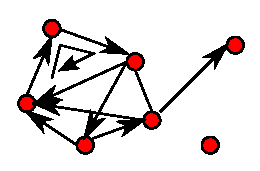
\includegraphics[width=5cm]{./figures/graph09.eps}
  \caption{Un graphe orienté avec un cycle.}
  \label{graph09}
\end{figure}

\begin{definition}[DAG]
  A \emph{directed acyclic graph} (DAG) is a directed graph without any cycle.
\end{definition}

\begin{definition}[topological order]
  Let $G=(V,E)$ a graph. $I$ is a \emph{topological order} if 
  \begin{itemize}
  \item $I$ is a bijection from $\lbrace1,\ldots,\rbrace$ to $V$
  \item \emph{If} $u$ is a parent of $v$, \emph{then} $I(u)<I(v)$
  \end{itemize}
\end{definition}

\begin{proposition}
  $G=(V,E)$ has a topological order $\Leftrightarrow$ $G$ is a DAG.
  \end{proposition}
\begin{proof}
$\Rightarrow$ easy,
$\Leftarrow$ use a depth-first search
\end{proof} 


\subsection{Directed graphical models}
\paragraph{Notations}
 $n$ discrete random variables $X_{1},\ldots,X_{n}$.
 \begin{itemize}
 \item joint distribution: $$p(x_{1},\ldots,x_{n})=P(X_{1}=x_{1},\ldots,X_{n}=x_{n})$$
\item marginal distribution: for $A\subset V$, $$p(x_{A})=p_{A}(x_{A})=P(X_{k}=x_{k},k\in A)=\sum_{x_{A^{c}}}
p(x_{A},x_{A^{c}})$$
\item conditional distribution: $$p(x_{A}|x_{A^{c}})=p_{A|A^{c}}(x_{A}|x_{A^{c}})=P(X_{A}=x_{A}|X_{A^{c}}=x_{A^{c}})$$
 \end{itemize}

\paragraph{Review}
$$\begin{array}{rcll}
X\independent  
Y&\Leftrightarrow& 
p(x,y)=p(x)p(y)& \forall x,y\\
&\Leftrightarrow&p_{XY}
(x,y)=p_{X}(x)p_{Y}(y)&\\
X\independent Y|
Z&\Leftrightarrow&p(x,y|
z)=p(x|z)p(y|z)& \forall 
x,y,z\\
&\Leftrightarrow &p(x|
y,z)=p(x|z)&
\end{array}$$


\subsubsection{Definitions and first properties} Let $G=(V,E)$ a DAG with $V=\lbrace1,\ldots n\rbrace$ and $(X_{1},\ldots,X_{n})$ $n$ discrete random variables. $ \mathcal{L}(G)$ set of $p(x)=p(x_{1},\ldots,x_{n})$ of the form $$p(x)=\prod_{i=1}^{n}f_{i}(x_{i},x_{\pi_{i}})$$ with\begin{itemize}
\item $\pi_{i}$ set of parents of $i$
\item $\forall i, f_{i}\geqslant0$
\item $\forall i,\sum_{x_{i}}f_{i}(x_{i},x_{\pi_{i}})=1$
\end{itemize} 

\begin{proposition}
If $p(x)$ factorizes in $G$,  i.e. $(p\in\mathcal{L}(G))$, then $p$ is a distribution and $$\forall i, f_{i}(x_{i},x_{\pi_{i}})=
p(x_{i}|x_{\pi_{i}})$$
\end{proposition}
\begin{proof}
By induction on $n=|V|$. See next class.

 \end{proof}


\end{document}
